\subsection{Drile world} 
 \subsubsection{Objects}
 In order to use the hierarchical live looping technique, the Drile implements several objects. This world tries to take the best part of the graphical interface.
\paragraph{Worms}    
 The first object is what we call a \textit{worm}. It is the representation of the nodes of the live-looping trees. They look like their associated analysed audio spectrum in order to ease the identification of each sound during a manipulation.
  
Those worms have graphical parameters such as color hue, size, transparency and so on. They are mapped to different audio effects parameters in such a way that modifying a worm's appearance would modify its audio effects. The current mapping are based on the result of a user study : size/volume, color hue/pitch, transparency/distortion, .. Moreover, the mapping is relative to each audio sample, so that each worms starts with the same appearance. To improve interaction a graphical parameter also gives the current value of the effect. The rotation of a worm on the y-axis provides information about the reading position of the associated audio.

\paragraph{Tunnels}    
Worms audio parameters and their associated graphical parameters can be modified by grabbing and sliding them through \textit{tunnels} as shown below \ref{fig:tunnel}. Each tunnel is used for one specific parameter modification.

\begin{figure}[h!]
\centering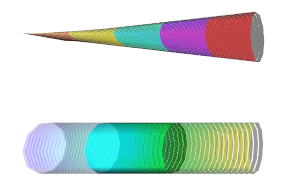
\includegraphics[scale=0.55]{image/tunnels.png}
\caption{Tunnels}
\label{fig:tunnel}
\end{figure} 

\paragraph{Hierarchy manipulation}  
As the size of worms is used to control node volume, manipulating worms through depth-axis would create perception problems. To settle that we use an \textit{interaction plane} which is at a fixed distance and allows manipulation of Drile objects. Depth-manipulations are maintained for less accurate uses.

Live-looping trees are represented by connected worms (\ref{fig:worm}) organized by depth. The closest level to the users is on the interaction plane.
Knowing that children nodes are the furthest from the user, accessing the different levels of the tree is possible by pulling and pushing the tree using Piivert gestures. 

\begin{figure}[h!]
\centering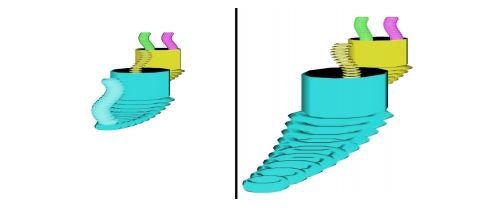
\includegraphics[scale=0.55]{image/worm.JPG}
\caption{Tree nodes containing colored worms. Appendages represent tree edges}
\label{fig:worm}
\end{figure} 

 Also, the user can take advantage of the 3D world by grabbing one worm directly with the ray-casting and then manipulating it. This can be facilitated with the head-tracking technique which simulate the fact of moving aside in front of a real scene and then it becomes easier to access objects in the back of the scene. 
 Common tree operations (merging, duplication, ..) are mapped to Piivert gestures that look natural to improve immersion. For example merging gesture is colliding two worms.

\paragraph{Scenes}  

During a performance, the user might want to use pre-built musical patterns, those ones are stored into \textit{scenes} (\ref{fig:scene}). He might also want to translate playing nodes from one to another scene in the aim of doing a nice musical transition. The 3D environnement creates a good visual feedback of the scene content which can help the user to choose the right scene.

\begin{figure}[h!]
\centering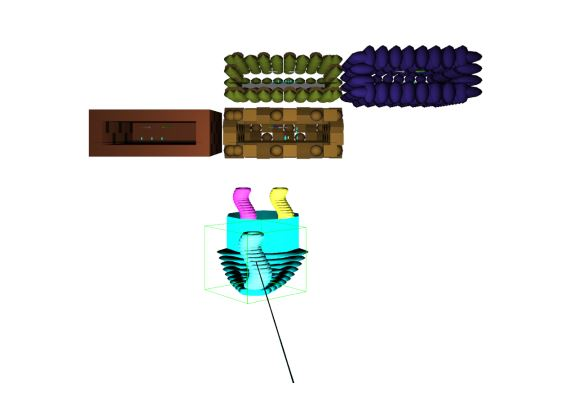
\includegraphics[scale=0.55]{image/scenes.JPG}
\caption{Scene selection for a worm translation}
\label{fig:scene}
\end{figure} 

\paragraph{Collaboration and Learning}

The Drile environnement is a multiple user interface as long as each user have one controller. The large display is also an advantage. As the Drile requires some expertise to have a proper handle on the music creation approach, two levels are implemented, one for beginners and one for experts. Beginners have access to higher level functions to learn the fundamental manipulations.

\paragraph{Evaluation of the instrument}

The author used a dimension space representation (\ref{fig:classinstr}) to evaluate his instrument according to \cite{birnbaum2005towards}. We can see that the Drile environnement fulfills two important sides in this representation : first the Feedback Modalities axe especially with the 3D environnement and the Piivert controller, secondly the Inter-Actors axe thanks to its multiple user interface and its large display.

\begin{figure}[h!]
\centering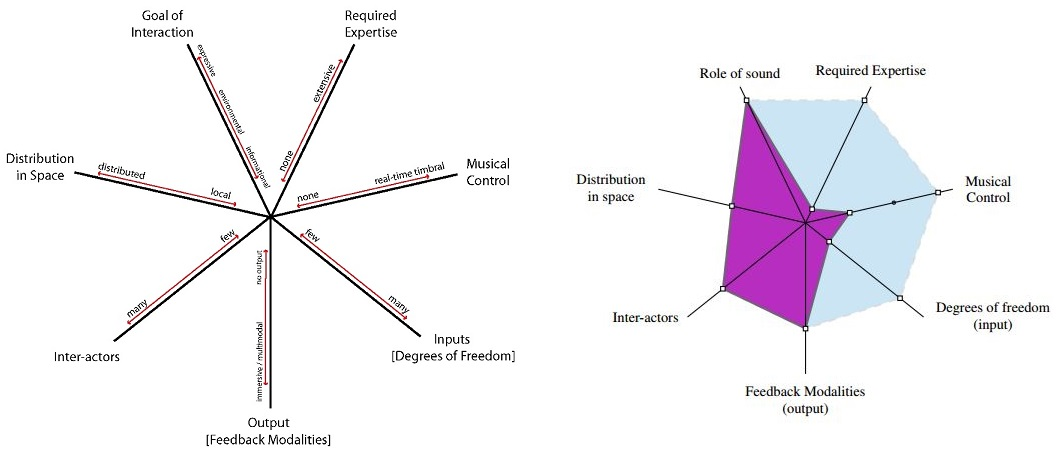
\includegraphics[scale=0.55]{image/classification_new_instr.jpg}
\caption{On the left the dimension space representation,
on the right the Drile representation (in purple for beginner interface, in blue for complete control)}
\label{fig:classinstr}
\end{figure} 


